\chapter{古典的情報、可逆な力学、そして行列}

\lectureoverview{量子力学は、通常の直観が鍛えられてきた範囲の外で推論することを我々に求める。そこで我々は一歩手前から、すなわち古典的情報——ビット、配置、可逆な更新則——から始める。同じ議論は自然にベクトルと行列へと導かれ、それらが量子ビットの言語を与えることになる。}

\section{誤った世界のために築かれた直観}

我々の物理的直観は古い。誰かが方程式を書くはるか以前から、獲物を追う動物は相対的な速さと方向を見積もらねばならなかった。ライオンがレイヨウに追いつきつつあるなら、ライオンは変化する間隔に反応しており、したがって暗黙のうちに相対速度に反応している。そのような判断をうまく扱う神経系が選ばれ、それをうまく扱えないものは多くの子孫を残さなかった。運動について我々が常識と呼ぶものの多くは、この日常世界で鍛えられたのである。

その遺産は有用だが、狭い。日常生活では何も光速に近い速さで動かないため、進化は相対論的時空に対する本能を与えなかった。物理学者はまず抽象的な幾何学を学び、その後になって初めてそれに対する新しい直観を獲得する。量子力学はさらに難しい。我々がよく知る粒子の像は石や矢から来ている。すなわち、各瞬間に物体は位置を持ち、位置の連なりが軌道をなし、位置の変化が速度を定義する。電子はその像に都合よく当てはまってはくれない。位置の不確定性と古典的軌道の不在は、我々の感覚を形作った経験の中に対応物を持たない。

この直観の失敗には逆説はない。逆説があるとすれば、石や動物や穏やかな速さに適応した本能が、どういうわけか電子について前もって知っていた場合だけである。正しい対応は、少数の精密な規則から別の直観を築くことである。ここでは、波動力学とSchr\"odinger方程式を通る通常の道筋を強調しない。我々は量子力学の論理構造と量子情報に集中する。量子ビットとは何かを問う前に、通常のビットが正確に何をするのかを理解しなければならない。

\section{ビットと情報量}

物理学は情報と切り離せない。その情報が実数で表されることもあるが、最も単純な情報は、二つの選択肢しかない問いへの答えである。すなわち、はいかいいえか、表か裏か、上か下かである。

\begin{definition}
\emph{古典的ビット}とは、ちょうど二つの可能な答えを持つ物理的な問いである。
\end{definition}

それらの答えを\(0\)と\(1\)とラベル付けしてよい。ラベルは本質的な意味を持たない。任意の二つの異なる記号で十分である。ディラック記法はまもなく不可欠になるので、まだ冗長であるうちに導入しておく。
\begin{equation}
  \ket{0},
  \qquad
  \ket{1}.
\end{equation}
縦棒と山括弧は\emph{ケット}を形成し、これはbra--ketの右半分である。記法を変えたからといって、量子論的なものは何も入ってきていない。

いくつかの区別可能なビットについては、答えを固定された順序で書く。例えば六つの区別可能なコインは、配置
\begin{equation}
  \ket{0\,1\,1\,0\,1\,0}.
\end{equation}
を持ちうる。順序が了解されれば、コンマは任意である。一つのビットは二つの可能な状態を持ち、二つのビットは四つを持ち、ビットを一つ加えるごとに数は倍になる。したがって\(n\)ビット系は
\begin{equation}
  N_s=2^n
  \label{eq:l01-state-count}
\end{equation}
個の状態を持つ。逆に、
\begin{equation}
  n=\log_2 N_s.
  \label{eq:l01-bits-from-states}
\end{equation}

式~\eqref{eq:l01-bits-from-states}は、状態の数が二の冪でない場合にも有用な定義を示唆する。
\begin{equation}
  I=\log_2 N_s.
  \label{eq:l01-information}
\end{equation}
したがって六面のサイコロは\(\log_2 6\)ビットの情報を担う。答えは整数である必要はない。文字通り二値スイッチから組み立てられた系は便利な例となるが、対数のほうがより一般的な尺度である。

\section{一見連続に見える世界の符号化}

ビットはコインに限られない。有限の精度で知られている任意の測定値は、有限の二進文字列として書くことができる。例えば、部屋の温度が選んだ有効数字の桁数までしか要求されないとしよう。測定値を二進法で表し、その精度に必要な桁を保持する。より高い精度にはより長い文字列が必要だが、原理の変更はない。

空間的に変化する場も同様に扱える。部屋を細かく順序付けられた格子状のセルに分割し、各セルの場の値を有限の精度で記録し、得られた二進文字列を連結する。セルを小さくすれば空間分解能が向上し、より多くの二進桁を保てば場の値の分解能が向上する。温度場、電場、磁場はいずれもこの方法で、任意に指定された有限の精度まで符号化できる。

粒子配置は、さらに文字通りの二値的な描像を与える。各セルが高々1個の粒子しか含まない程度に細かく空間を分割する。次を割り当てる。
\begin{equation}
  n_i=
  \begin{cases}
    1,&\text{cell \(i\) is occupied},\\
    0,&\text{cell \(i\) is empty}.
  \end{cases}
  \label{eq:l01-occupancy-bit}
\end{equation}
完全な配置は順序付けられた文字列である。
\begin{equation}
  \ket{n_1n_2n_3\cdots}.
\end{equation}
これは、はい・いいえの質問の並びに対する非常に長い答えである。すなわち、最初のセルに粒子はあるか、二番目のセルにはあるか、以下同様に問うのである。これはゲーム\emph{二十の質問}の物理版にほかならないが、質問の数が膨大になりうる点が異なる。

この構成は、デジタル計算機がなぜ物理をシミュレートできるのかを説明する。計算機は有限の文字列を記憶し、一方、有限の分解能は測定された量や場をまさにそのような文字列に変える。近似は、格子、時間刻み、または保持する桁数を細かくすることによって系統的に改善できる。

\begin{classroomqa}
\lecturetimestamp{00:29:43}
\audiencequestion{温度の表現の精度は任意なのですか。}
\lecturerresponse{それは、我々が望む近似に応じて選ばれる。有限の文字列は有限の精度を与え、より多くの二進桁を保持すればより細かい近似が得られる。ここで主張しているのは、有限の文字列が任意の古典的実数を正確に指定するということではない。}
\end{classroomqa}

\begin{classroomqa}
\lecturetimestamp{00:30:11}
\audiencequestion{一般の実数、特に無理数の場合はどうなるのですか。}
\lecturerresponse{正確な実数は無限に多くのビットを必要とすることがある。有理数の二進展開には循環するものがあり、一般の無理数の展開は決して終わらない。実在の計算機は常に有限個の桁しか保持しない。要点は、指定された任意の有限精度を符号化できるということであり、すべての古典的実数が有限の正確な記述をもつということではない。}
\end{classroomqa}

\section{状態と運動法則}

これまでは、ある一瞬における系を記述してきた。運動には第二の要素が必要である。

\begin{definition}
\emph{配置}とは、指定された一瞬における系の完全な状態である。離散時間の運動法則とは、各配置を1時間ステップ後の配置へ写す規則である。
\end{definition}

この区別は初歩的だが本質的である。電子分布のスナップショットは配置であり、まだ軌道ではない。空間を格子に、時間を数列\(t_0,t_1,t_2,\ldots\)に置き換えるなら、運動は次の連なりである。
\begin{equation}
  \ket{s(t_0)}
  \longmapsto
  \ket{s(t_1)}
  \longmapsto
  \ket{s(t_2)}
  \longmapsto\cdots.
  \label{eq:l01-discrete-motion}
\end{equation}
したがって物理模型には、可能な状態の集合と更新規則の両方が必要である。

\begin{classroomqa}
\lecturetimestamp{00:31:12}
\audiencequestion{このセルによる記述は、軌道を運動する電子をどのように説明するのですか。}
\lecturerresponse{まず、ある一瞬における配置だけを指定する。どのセルが占有されているかであり、それが模型の一部なら原子核は固定しておく。次に時間を離散化する。軌道運動は、ある占有文字列を次の文字列へ更新する規則である。セルの順序付けのためにその規則は複雑になりうるが、それでも情報の更新には変わりない。}
\end{classroomqa}

抽象的な\emph{状態空間}を描くと助けになる。この空間の各点は、通常の空間内の位置ではなく、配置全体を表す。\(10\times10\)の占有格子は百ビットを含み、したがって\(2^{100}\)個の可能な配置をもつ。\editorialnote{講義の音声ではこの例を展開する際に一時的に\(10^{100}\)と言っているが、ビット数から意図された値は\(2^{100}\)であると確定する。}それら各配置の一つ一つが、状態空間における単一の点である。

1ビットの場合、点は二つしかない。恒等法則は両方を固定する。
\begin{equation}
  0\mapsto0,
  \qquad
  1\mapsto1.
  \label{eq:l01-identity-update}
\end{equation}
もう一つの可逆な可能性は両者を入れ替える。
\begin{equation}
  0\mapsto1,
  \qquad
  1\mapsto0.
  \label{eq:l01-flip-update}
\end{equation}
これはフリップフロップである。自由に発展する物理的な例は、手で操作する照明スイッチよりもすぐには思いつかない。介入すれば系が拡大されてしまうからである。昼と夜は近似的な二状態の周期を与え、振り子も両極端の間を交互に往復するが、その完全な状態にはすべての中間の位置と速度が含まれる。

\begin{classroomqa}
\lecturetimestamp{00:40:38}
\audiencequestion{普通の照明スイッチはフリップフロップ法則の例になるのですか。}
\lecturerresponse{人がそれを切り替えているのであれば、そうではない。その場合、スイッチは自ら発展しているのではなく、人が拡大された力学系に属するからである。我々が求めるのは、自らの法則がその状態を交互に変える閉じた系である。昼と夜はその考えを示唆し、振り子は、実際の例が通常は二つより多くの状態をもつことを思い出させる。}
\end{classroomqa}

2ビットの系には四つの配置がある。一つの更新法則は四つすべてを単一の周期に沿って巡らせてもよい。別の法則は二つの別々の二周期からなってもよい。これらは配置の論理空間におけるループであり、必ずしも物理空間におけるループではない。矢印が法則を指定する。系がどこから始まっても、矢印をたどればその後の履歴がわかる。

\section{可逆性と区別の保存}

すべての矢印図が同じ物理的状態をもつわけではない。二つの異なる状態が同じ後続状態に合流する規則を考えよう：
\begin{equation}
  a\mapsto c,
  \qquad
  b\mapsto c.
  \label{eq:l01-merging-update}
\end{equation}
\(a\)から出発しても\(b\)から出発しても次の状態は定義されるが、\(c\)に到達した後では、どちらの過去が起こったのかを決定できない。\(a\)と\(b\)の区別は消えてしまった。

\begin{figure}[htbp]
\centering
\includegraphics[width=0.82\linewidth]{lecture_01_figure_02.png}
\caption{可逆性の議論の間、いくつかの更新図が黒板に残っている。閉じたサイクルが合流パターンと共存し、量子論の用語\emph{ユニタリティ}がそれらのそばに書かれている。}
\lectureframe{00:53:21}
\end{figure}

\begin{figure}[htbp]
\centering
\begin{tikzpicture}[>=Latex,thick,node distance=1.15cm]
  \node[circle,fill,inner sep=1.8pt,label=above:\(1\)] (r1) {};
  \node[circle,fill,inner sep=1.8pt,right=of r1,label=above:\(2\)] (r2) {};
  \node[circle,fill,inner sep=1.8pt,below=of r2,label=below:\(3\)] (r3) {};
  \node[circle,fill,inner sep=1.8pt,left=of r3,label=below:\(4\)] (r4) {};
  \draw[->] (r1) -- (r2);
  \draw[->] (r2) -- (r3);
  \draw[->] (r3) -- (r4);
  \draw[->] (r4) -- (r1);
  \node[below=0.5cm of r4,anchor=north west] {\small reversible cycle};

  \node[circle,fill,inner sep=1.8pt,right=4.2cm of r1,label=above:\(a\)] (a) {};
  \node[circle,fill,inner sep=1.8pt,below=1.25cm of a,label=below:\(b\)] (b) {};
  \node[circle,fill,inner sep=1.8pt,right=1.6cm of a,yshift=-0.625cm,label=above:\(c\)] (c) {};
  \node[circle,fill,inner sep=1.8pt,right=of c,label=above:\(d\)] (d) {};
  \draw[->] (a) -- (c);
  \draw[->] (b) -- (c);
  \draw[->] (c) -- (d);
  \node[below=0.55cm of b,anchor=north west] {\small information-losing merge};
\end{tikzpicture}
\caption{可逆な規則は各状態に一つの先行状態と一つの後続状態を割り当てる。合流規則は一意な未来をもつが、過去は曖昧である。}
\end{figure}

基礎的な古典力学は、すべての自由度が保持されている場合にはこの損失を許さない。要求される性質には二つの側面がある：
\begin{equation}
  \boxed{\begin{gathered}
    \text{one unique future and one unique past}\\
    \text{for every state}
  \end{gathered}.}
  \label{eq:l01-reversibility}
\end{equation}
有限の状態空間に対しては、したがって更新は置換でなければならない。各状態はちょうど一つの出ていく矢印とちょうど一つの入ってくる矢印をもつので、図は互いに素なサイクルに分解される。

\begin{classroomqa}
\lecturetimestamp{00:46:32}
\audiencequestion{合流図の何が異なるのか？}
\lecturerresponse{それは完全にループから成るわけではない。より根本的には、系が合流状態にあるのを見つけても、それがどの先行状態をもっていたかを教えてくれない。未来は構成できるが、過去は再構成できない。歴史的区別の1ビットが失われている。}
\end{classroomqa}

この概念は\emph{時間可逆性}であり、必ずしも厳密な時間反転対称性ではない。時計回りのサイクルは明確な前向きの向きをもつ。元の法則は系を反時計回りに送らないが、そうする逆法則が存在する。厳密な時間反転対称性は追加の問いを立てる：適切な反転操作を適用した後、同じ力学法則が得られるか？ 可逆性だけは、歴史を一意に逆にたどれるかどうかだけを問う。

\begin{classroomqa}
\lecturetimestamp{00:49:58}
\audiencequestion{過去の一意性は単に時間反転対称性なのか？}
\lecturerresponse{厳密にはそうではない。サイクルの矢印は一方向だけを指すことがあり、したがって法則には向きがある。可逆性とは、すべての矢印を逆にすることで明確に定義された逆法則を構成できることを意味する。それは逆法則が元の法則と同一であること自体を述べているのではない。}
\end{classroomqa}

また、合流状態に二つの出ていく矢印を置くことで不可逆な図を修復すべきでもない。それは逆方向の運動を別の仕方で曖昧にするであろう：系は確率的な指示を必要とし、おそらく\(30\%\)の確率で一方の枝を、\(70\%\)の確率で他方の枝を選ぶであろう。われわれは依然として決定論的な古典力学を構成しており、そこでは一つの現在状態が一つの未来と一つの過去を決定する。

すべての実在系は究極的には量子力学的である。なぜ大きな物体が古典的に見えるのか、なぜそれらの量子的な選択肢が観測しにくくなるのかは、後の問題である。対応する量子原理は同じ論理的核心を保つであろう。半ば冗談で、過去と未来の一意性を\emph{ユニークタリティ}と呼ぶかもしれない。その実際の名前は\emph{ユニタリティ}である：量子進化は一意に前向きにも後向きにも進めることができる。

\section{見かけの情報損失と粗視化}

巨視的な経験は可逆性と矛盾するように見える。密閉された部屋の左隅に気体のすべての分子を集めて放す。まもなく気体は部屋を満たす。代わりに右隅から始めても、最終的な巨視的描像は同じに見える。二つの異なる初期状態は合流したのか？

詳細を捨て去った後にのみそうなる。微視的状態はすべての分子を指定する。すべての位置と速度を十分な精度で追跡できれば、それらの運動を逆転させることで二つの準備を区別できるであろう。実際には計算は法外に難しく、必要な精度は急速に増大するが、実際的な不能は根本的な消去ではない。巨視的な記述\emph{空気が部屋を満たす}は、膨大な数の異なる微視的配置を一つの粗視化状態として同定する。

ここで熱力学第二法則が入ってくる。詳細な状態を区別する能力を失うのは、すべての微視的変数を追跡しないからである。情報が見かけ上消えるのは、われわれの記述が粗いからであり、細粒子的な決定論的法則が異なる点を合流させるからではない。

\begin{classroomqa}
\lecturetimestamp{00:56:11}
\audiencequestion{古典的な部屋のすべての分子を追跡するには無限個のビットが必要だろうか。}
\lecturerresponse{厳密な古典的記述のためには、そうである。位置と速度は実数であり、カオス的な多粒子系をより長い時間にわたって追跡するには、ますます高い精度が要求される。量子力学はこの結論を変える。エネルギーが有界な閉じた領域では、物理的に区別可能な記述は、古典的な厳密な実数の任意のリストではなく、離散的でありうる。}
\end{classroomqa}

この問題は単に学術的なものではない。ブラックホールが情報を破壊しうるかどうかは何十年にもわたって論争されてきた。スティーブン・ホーキングは当初、破壊しうると主張した。この論争は、見かけの合体が単に別の粗視化された記述にすぎないのか、それとも量子ユニタリティの真の破れなのかを問うものである。量子力学が正確な言語を与える前にこれを決着させることはしないが、この論争は、単純な矢印の図にどれほど多くがかかっているかを明らかにしている。

\section{行、列、内積}

古典的ビットを量子ビットに置き換える前に、少しばかり線形代数が必要である。当面の目的には、ベクトルは単に実数の有限な順序付きリストとみなしてよい。4成分ベクトルは横に、
\begin{equation}
  A^{\mathsf T}=(A_1,A_2,A_3,A_4),
  \label{eq:l01-row-vector}
\end{equation}
または縦に、
\begin{equation}
  A=
  \begin{pmatrix}
    A_1\\ A_2\\ A_3\\ A_4
  \end{pmatrix}.
  \label{eq:l01-column-vector}
\end{equation}
書くことができる。\emph{4次元}という語は、成分が4つあるというだけの意味である。通常の空間における矢印を思い描く必要はない。横に書いたものは行ベクトルであり、縦に書いたものは列ベクトルである。

\begin{figure}[htbp]
\centering
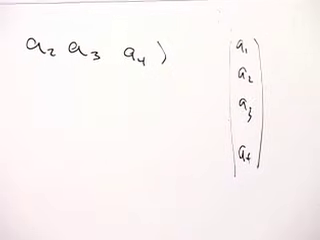
\includegraphics[width=0.92\linewidth]{lecture_01_figure_03.png}
\caption{同じ成分が行としても列としても書かれている。この段階ではそれらは実数であるから、複素共役は関与しない。}
\lectureframe{01:03:05}
\end{figure}

\begin{classroomqa}
\lecturetimestamp{01:03:14}
\audiencequestion{行ベクトルは列ベクトルのダガーではないのか。}
\lecturerresponse{成分が複素数になれば、それが正しい言語となる。そのときには転置に複素共役が伴わなければならない。今のところ成分は実数であるから、行の配置と列の配置を区別するだけでよい。}
\end{classroomqa}

列\(A\)と同じ個数の成分をもつ行を
\begin{equation}
  B=(B_1,B_2,B_3,B_4)
\end{equation}
とする。それらの積は、位置を対応させて和をとることにより定義される。
\begin{align}
  BA
  &=
  (B_1,B_2,B_3,B_4)
  \begin{pmatrix}
    A_1\\ A_2\\ A_3\\ A_4
  \end{pmatrix}\\
  &=B_1A_1+B_2A_2+B_3A_3+B_4A_4.
  \label{eq:l01-inner-product}
\end{align}
結果は数であり、別のベクトルや行列ではない。抽象ベクトル空間において、この演算は内積と呼ばれる。

\begin{classroomqa}
\lecturetimestamp{01:06:44}
\audiencequestion{これはドット積か。}
\lecturerresponse{はい。3次元空間における通常のベクトルに対しては、それはよく知られたドット積である。\emph{内積}という名は、同じ行と列の積の演算が任意の有限次元のベクトル空間に適用されることを強調している。}
\end{classroomqa}

\section{状態を更新する機械としての行列}

行列とは、ベクトルに作用して別のベクトルを生み出す、数の正方形配列である。これを機械のように考えるとよい。古い列を入力し、固定された規則を適用して、新しい列を得る。4次元では、
\begin{equation}
  M=
  \begin{pmatrix}
    M_{11}&M_{12}&M_{13}&M_{14}\\
    M_{21}&M_{22}&M_{23}&M_{24}\\
    M_{31}&M_{32}&M_{33}&M_{34}\\
    M_{41}&M_{42}&M_{43}&M_{44}
  \end{pmatrix}.
  \label{eq:l01-general-matrix}
\end{equation}
第1の添字は行を、第2の添字は列を表す。\(M\)は列の集まりと見ることも、行の集まりと見ることもできる。どちらの見方も有用である。

\(A'=MA\)を計算するには、\(M\)の各行と入力列との内積を取る。
\begin{equation}
  A'_i=(MA)_i=\sum_{j=1}^{4}M_{ij}A_j.
  \label{eq:l01-matrix-vector}
\end{equation}
例えば、
\begin{align}
  A'_1&=M_{11}A_1+M_{12}A_2+M_{13}A_3+M_{14}A_4,\\
  A'_2&=M_{21}A_1+M_{22}A_2+M_{23}A_3+M_{24}A_4.
\end{align}
第3および第4の成分も同じパターンで従う。

\begin{figure}[htbp]
\centering
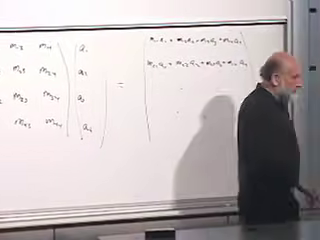
\includegraphics[width=0.94\linewidth]{lecture_01_figure_04.png}
\caption{行列は列ベクトルに各行ごとに作用する。最初の2つの出力成分が黒板で明示的に展開されている。}
\lectureframe{01:12:45}
\end{figure}

\subsection{古典的配置の符号化}

系が4つの可能な状態をもつとしよう。それらをワンホット列
\begin{equation}
  e_1=
  \begin{pmatrix}1\\0\\0\\0\end{pmatrix},
  \quad
  e_2=
  \begin{pmatrix}0\\1\\0\\0\end{pmatrix},
  \quad
  e_3=
  \begin{pmatrix}0\\0\\1\\0\end{pmatrix},
  \quad
  e_4=
  \begin{pmatrix}0\\0\\0\\1\end{pmatrix}.
  \label{eq:l01-one-hot}
\end{equation}
で表す。単一の\(1\)の位置が、どの古典的配置が存在するかを教えてくれる。

巡回更新
\begin{equation}
  1\longrightarrow2\longrightarrow3\longrightarrow4\longrightarrow1.
  \label{eq:l01-four-cycle}
\end{equation}
を考えよう。それは
\begin{equation}
  P=
  \begin{pmatrix}
    0&0&0&1\\
    1&0&0&0\\
    0&1&0&0\\
    0&0&1&0
  \end{pmatrix}.
  \label{eq:l01-permutation-matrix}
\end{equation}
で表される。実際、
\begin{equation}
  \begin{aligned}
    Pe_1&=e_2, & Pe_2&=e_3,\\
    Pe_3&=e_4, & Pe_4&=e_1.
  \end{aligned}
\end{equation}
黒板での構成は書かれている途中で訂正され、まず5つの状態で、次に4つの状態で行われる。式~\eqref{eq:l01-permutation-matrix}は、放棄された中間の配列ではなく、確定した巡回規則を記録している。

同じ行列が任意の列に作用する。
\begin{equation}
  P
  \begin{pmatrix}A\\B\\C\\D\end{pmatrix}
  =
  \begin{pmatrix}D\\A\\B\\C\end{pmatrix}.
  \label{eq:l01-cyclic-shift}
\end{equation}
古典的状態ではただ1つの成分だけが\(1\)であるが、一般の成分を許すことで、その背後にある線形演算が明らかになる。古典的決定論的更新は、すべての行とすべての列に\(1\)を1つずつもつ特別な0-1行列を用いる。量子力学は、許される成分を大幅に拡大しつつ、行列による発展を保持するであろう。

\subsection{合成は行列の積である}

1ステップの時間発展が
\begin{equation}
  V'=MV,
\end{equation}
であるならば、2回目の適用により
\begin{equation}
  V''=MV'=M(MV)=M^2V.
  \label{eq:l01-two-updates}
\end{equation}
が得られる。したがって、行列の乗算は恣意的な代数的遊びではない。それは物理的な更新を合成する。5ステップの時間発展は\(M^5\)で表される。

2つの \(2\times2\) 行列
\begin{equation}
  M=
  \begin{pmatrix}
    M_{11}&M_{12}\\
    M_{21}&M_{22}
  \end{pmatrix},
  \qquad
  N=
  \begin{pmatrix}
    N_{11}&N_{12}\\
    N_{21}&N_{22}
  \end{pmatrix},
\end{equation}
に対して、積 \(C=MN\) の成分は
\begin{equation}
  C_{ij}=\sum_k M_{ik}N_{kj}.
  \label{eq:l01-matrix-product}
\end{equation}
である。特に、
\begin{align}
  C_{11}&=M_{11}N_{11}+M_{12}N_{21},\\
  C_{12}&=M_{11}N_{12}+M_{12}N_{22},\\
  C_{21}&=M_{21}N_{11}+M_{22}N_{21},\\
  C_{22}&=M_{21}N_{12}+M_{22}N_{22}.
\end{align}
各成分は、左の行列の行と右の行列の列を掛けたものである。同値に、\(M\) を \(N\) の各列に作用させ、得られた列を横に並べてもよい。

\begin{figure}[htbp]
\centering
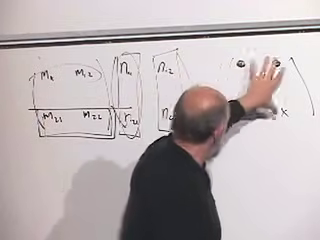
\includegraphics[width=0.86\linewidth]{lecture_01_figure_05.png}
\caption{行列の積を、行列--列の乗算の繰り返しとして整理したもの。積の各成分の由来を示すため、第1行と第2の行列の各列に印が付けられている。}
\lectureframe{01:26:30}
\end{figure}


行ベクトルも左から作用できる。\(B=(B_1,\ldots,B_4)\) ならば、\(BM\) は別の行ベクトルであり、
\begin{equation}
  (BM)_j=\sum_i B_iM_{ij}.
  \label{eq:l01-row-times-matrix}
\end{equation}
である。ここでも規則は行×列である。形が結果を追跡する：
\begin{equation}
\begin{array}{c@{\qquad}c}
\text{row}\times\text{column}&=\text{number},\\
\text{matrix}\times\text{column}&=\text{column},\\
\text{row}\times\text{matrix}&=\text{row},\\
\text{matrix}\times\text{matrix}&=\text{matrix}.
\end{array}
\label{eq:l01-shape-rules}
\end{equation}

これらの演算は、小さな数値の \(2\times2\) および \(3\times3\) の例で練習する価値がある。少しの微積分とともに、行--列の積は、この先の量子力学に必要な主要な新しい数学的習慣である。

\begin{classroomqa}
\lecturetimestamp{01:31:50}
\audiencequestion{可逆性は更新行列にどのような制限を課すか？}
\lecturerresponse{それは逆行列を持たなければならない。逆行列は逆の更新を実装し、すべての状態をその一意な先行状態へ戻す。すべての行列が可逆であるわけではないので、この代数は以前に矢印図で行った区別を再現する。巡回的な例では、\(P^{-1}=P^3\) および \(P^4=\mathbb{1}\) である。}
\end{classroomqa}

\section{なぜ量子ビットの前に代数を準備するのか？}

最初の1時間では、ビットと可逆な矢印を用いて、決定論的な古典物理学を定性的に説明した。残りの数学は、その説明を量子力学への移行に耐えうる形に翻訳する。配置は列になり、1ステップの法則は行列になり、繰り返される時間発展は行列の積になり、可逆性は逆行列の存在になる。

まだ量子規則は使っていない。この遅延は意図的である。次に、古典的な選択肢 \(\ket{0}\) と \(\ket{1}\) を量子ビットに置き換え、どのような新しい状態が可能かを問う。ここで導入した行ベクトル、列ベクトル、内積、行列は、そのとき、量子情報が古典的なビット列といかに鋭く異なるかを明らかにするだろう。

\begin{classroomqa}
\lecturetimestamp{01:34:00}
\audiencequestion{なぜそれが何のためかを言う前に、これほど多くの行列代数を導入するのか？}
\lecturerresponse{定性的な問題が先に来た：決定論的物理学は状態と更新法則によってどのように表されるべきか？この代数は次の段階への準備である。量子ビットが導入されれば、これらの操作はもはや無関係には見えず、量子状態とその発展の自然な言語となるだろう。}
\end{classroomqa}